\chapter{Week}
\section{Data set collection}
The final data set collection amounted to 11503 images with a distribution of 2838 images for the 'ROCK' class, 2820 images for the 'PAPER' class, 2814 images for the 'SCISSORS' class and 2749 images for the 'ILLEGAL' symbol class. The 'BACKGROUND' class consists of 282 images. To add to this number a publicly available data set was also added to the collection containing 2188 images in total distributed almost equally amongst the classes 'ROCK', 'PAPER' and 'SCISSORS'. The complete data set was then handed of to Synthara for the training process as agreed when starting the collaboration. The data set was augmented as described in the chapter before and then iteratively quantized to compress the network.
\section{Robot hand ordering}
As the training process would take up to two weeks at least, the next reasonable step was to work on the hardware setup with the Enclustra board. A crucial part for this is the robotic hand. At first, I conducted research into the available possibilities: There are numerous options ranging from cheap ($\sim 50$ \$) servo motor controlled basic hands to more sophisticated 3D-printed medical variants (several thousand \$). For this demonstrator the key parameter was speed, so that the robot hand would react in time to the classification results provided by the neural network. The key parameter for this is how quickly the attached servos can go from 0 $^\circ$ to 180 $^\circ$. The typical value for this is around 1 to 2 $ms$ for the cheaper robotic hands. The more expensive 3D printed ones were taken out of consideration because of the cost.
\begin{figure}[!htb]
	\centering
		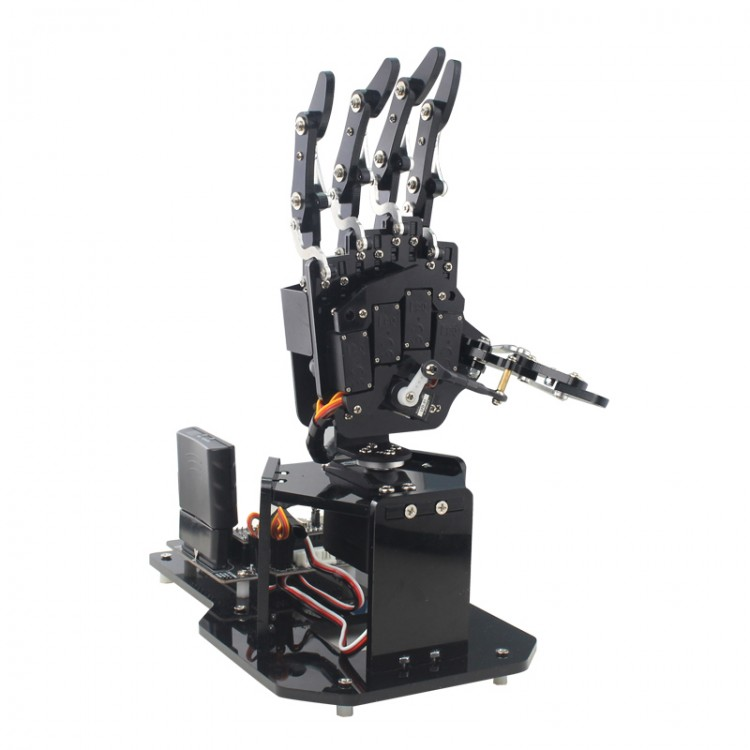
\includegraphics[width=\textwidth]{bilder/robohand.jpg}
		\caption{Robotic hand chosen for the demonstrator}
		\label{fig:robohand}
\end{figure}
Figure~\ref{fig:robohand} shows the chosen robotic hand. The benefits of this system is the added \ac{PCB} together with a microcontroller, so that the basic functionality can be tested easily and directly. The servos used in this hand are very standard servo motors with three connectors, VCC, GND and DATA. The DATA line is used to determine the angle which the servo has to drive to. The signal used for this is a \ac{PWM}. Figure~\ref{fig:pwm_servo} shows the mapping of the \ac{PWM} signal to the motor position.
\begin{figure}[!htb]
	\centering
		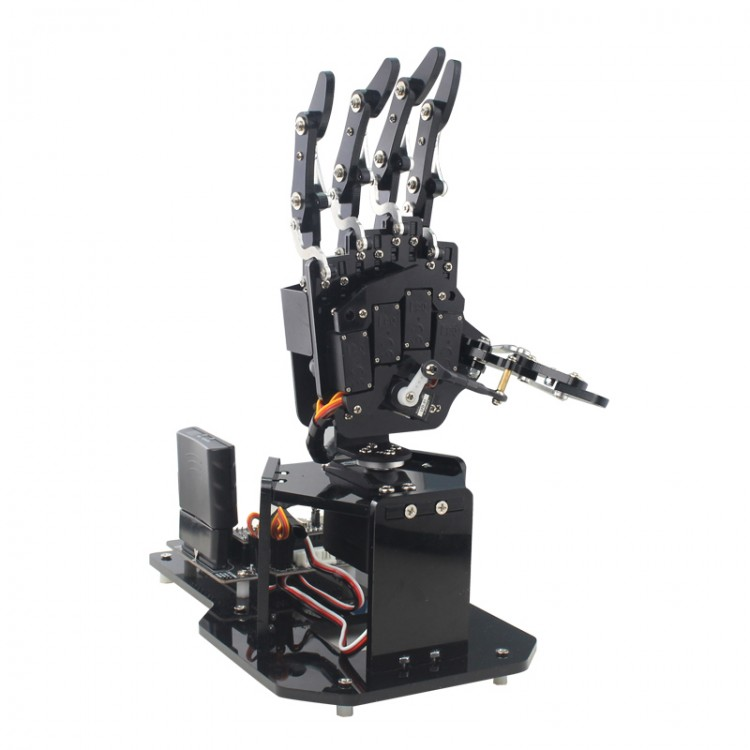
\includegraphics[width=\textwidth]{bilder/robohand.jpg}
		\caption{\acs{PWM} signal servo motor position mapping}
		\label{fig:pwm_servo}
\end{figure}
\section{Internship documentation}
The rest of the week was spent on writing documentation of all of the tasks I completed during my internship so far and integrate this information into the company Wiki.